\section{Implementation Plan}
The Architectural Styles and Patterns of the system to be are huge explained in Section \ref{architecturalStyle}.\\
The implementation of our system will be done module by module and component by component, most relevant and complex part of the system to be is the \textit{Controller} of the MVC model.\\
The developing of the modules must be done keeping attention in writing good \textit{Documentation of the Code}, doing \textit{Unit test} and
finally making \textit{Code Inspection and Analysis}; these topics are explained in the Section \ref{int_test}.\\
Below there is a Figure in order to explain the implementation flow, several detailed on the \textit{Application Server} components that are the huge part of the \textit{Controller}.

\begin{figure}[H]
  \begin{center}
  	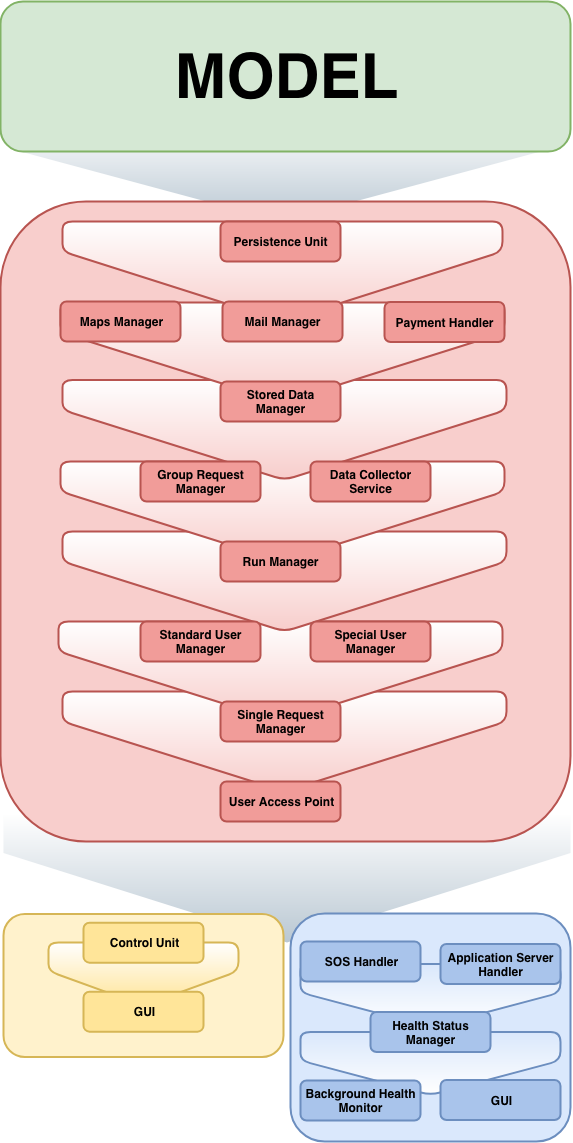
\includegraphics[height=0.59\paperheight]{./img/implementationFlow.png}
    \hspace{0.05\linewidth}
    \centering
    \caption{\textit{Implementation Plan} of the system}
		\label{img:implementationFlow}
    \end{center}
\end{figure}

\subsection{Implementation Plan Discussion}
\myparagraph{}
The \textit{Model} is the first part of the system the must be implemented. This choice is supported by the facts that the \textit{Model} is used by most of the components in the \textit{Application Server} and some part of it are represented in the \textit{Database} avoiding any type of duplication or confusion between what we consider \textit{Model} and \textit{Controller} is the main motivation of this choice.

\myparagraph{}
The second most relevant part of the system that must be developed is the \textit{Controller}, and we find in it components of the \textit{Application Server}.
\begin{itemize}
  \item \textbf{Persistence Unit} is the first component of this part that must be implemented because it manages all communication with the DBMS and communicates with a large part of the components in this part of the system.
  \item \textbf{Maps Manager}, \textbf{Mail Manger} and \textbf{Payment Handler} are components the provides the majority of services in common among other components and \textit{Maps Manager} and \textit{Payment Handler} also are the components that interfaces with the external services.
  \item \textbf{Stored Data Manager} is a critical component: it allows to manage data about users, it receives and sends data. It has an important role in data request; it provides interface for other components, for these reasons it must be developed alone.
  \item \textbf{Group Request Manager} and \textbf{Data Collector Service} provides some of the services provides by \textit{Data4Help}. They are at the base of other components so their implementation must be done keeping attention.
  \item \textbf{Run Manager} is the component that allows our system to manage the \textit{Run}'s services, fault tollerance must be guarantee. It is the core of this service and its implementation is crucial. It also provides an interface to the \textit{Standard User Manager} components and it use the \textit{Maps Manager}. component.
  \item \textbf{Standard User Manager} and \textbf{Special User Manager} are the core all actions performed by a \textit{Generic User} of \textit{Data4Help}. They communicate with most of the components described before and their implementation has to guarantee very high tolerance to fault and good performance because they represent a possible bottleneck of the application.
  \item \textbf{Single Request Manager} like some previous components it provides one of the core service of \textit{Data4Help}. Its implementation is inserted at this point because it requires some important functionalities of \textit{Standard User Manager} and \textit{Special User Manager}.
  \item \textbf{User Access Point} main function is to redirect users and their requests. It provides a way to communicate with the the internal components.
\end{itemize}

\myparagraph{}
It is the last part of the system to be that must be implemented and needs the main functionalities of the \textit{Controller}.\\
The flow of implementation of the internal components \textit{AutomatedSOS} is specified to avoid any possible problems, being a critical service.

\subsection{Implementation Choices}

\subsubsection{Database}
The choice of the \textit{Database} is MySQL 5.7 as relational DBMS and InnoDB as Database Engine. This last choice is to manage concurrency accessing same tables.

\subsubsection{Application Server}
The implementation of this important layer is the use of Java Enterprise Edition 7 (JEE) with a GlassFish Server. Java Persistence API (JPA) is used to interface with the DBMS, JAX-RS to implement RESTful APIs to interface with mobile application, \textit{Web Server} and also with the \textit{External Servicies}.

\subsubsection{Mobile App}
The mobile applications must be implemented in two different architecture respecting native languages, Swift for iOS application and Java for Android ones. The communication with the device must be done using the default frameworks of the respective system, moreover the communication with the \textit{Application Server} and \textit{External Services} must be performed with RESTful APIs.

\subsubsection{Web Server}
As we decided to implement the \textit{Application Server} with JEE, that choice is reflected to this layer. We have only to specify that the implementation of the \textit{GUI} must be performed with HTML5 and CSS; \textit{Control Unit} using JavaServer Pages (JSP).

%TODO Implementation Tree

\section{Integration and Testing}\label{int_test}

\subsection{Entry Criteria}

\subsubsection{Integration Testing Strategy}

\subsubsection{Integration Sequence}
